\title{Lecture 1: Set}
\frame{\titlepage}



%%%%%%%%%%%%%
\section{Concept}
\frame{\sectionpage}
%%%%%%%%%%%%%

\begin{frame}
\frametitle{Rough definition}
\begin{block}{}
A \textbf{set} is a box that contains things.
\end{block}
\begin{description}
\item[Object] collection, group, gathering, category, container, box, circle, area, boundary 
\item[Complement] outside, different 
\item[Operation] add, combine, subtract, take away, remove, exclude 
\item[Comparison] differentiate, distinct, distinguish, outstanding, outlier 
\end{description}
\end{frame}

\begin{frame}{Formal set notation (1/2)}
\begin{defn}{Definition of Set}{}
A \textbf{set} is a collection of distinct objects (called \textbf{elements} or \textbf{members}). 
\begin{itemize}
\item Sets are usually denoted by capital letters ($A, B, C$).
\item Enclosed in curly braces: e.g., $A = \{1, 2, 3, 5, \text{apple}\}$.
\end{itemize}
\tcblower
\textbf{Membership Notation:}
\begin{itemize}
\item If $x$ is an element of $A$, we write $x \in A$ ($x$ is in $A$). 
\item If not, we write $x \notin A$ ($x$ is not in $A$). 
\item Example: For $A = \{1, 2, 3\}$, we have $1 \in A$ and $4 \notin A$.
\end{itemize}
\end{defn}
\end{frame}

\begin{frame}{Formal set notation (2/2)}
\begin{block}{Key Properties of Sets}
\begin{enumerate}
\item \textbf{Order doesn't matter:}
\[ \{1, 2, 3\} = \{2, 1, 3\} \]
\textit{Why?} A set is defined strictly by \textbf{membership} (what belongs to it). Testing whether $x \in A$ gives the exact same result regardless of element order. 

\item \textbf{Duplicate items don't matter:}
\[ \{1, 2, 3, 3, 2, 1\} = \{1, 2, 3\} \]
\textit{Why?} A set tracks \textbf{existence} (presence or absence), not quantity/count. An object either belongs to the set ($x \in A$) or does not ($x \notin A$); repeating it does not alter membership status.
\end{enumerate}
\end{block}
\end{frame}

\begin{frame}{Reading Set Diagrams}
\begin{columns}
\begin{column}{0.52\textwidth}
\begin{block}{How to Read a Diagram}
\begin{itemize}
\item \textbf{Inside circle:} Elements in set ($x \in A$).
\item \textbf{Outside circle:} Non-elements ($y \notin A$).
\item From figure: $A = \{-2, 0, 1, 3\}$ and $4 \notin A$.
\end{itemize}
\end{block}
\end{column}
\begin{column}{0.48\textwidth}
\begin{figure}[h!]
\centering
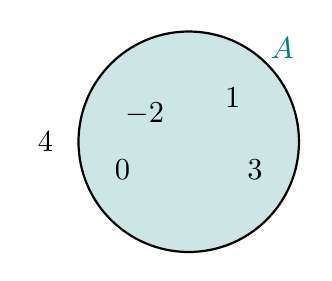
\begin{tikzpicture}[scale=0.7, every node/.style={scale = 1.1}]
\filldraw[fill = teal!20, draw = black, thick] (0,0) circle (2cm);
\node at (0.8,0.8) {$1$};
\node at (1.2,-0.5) {$3$};
\node at (-0.8,0.5) {$-2$};
\node at (-1.2,-0.5) {$0$};
\node at (-2.6,0) {$4$};
\node[teal] at (45: 2.4)  {\textbf{$A$}};
\end{tikzpicture}
\caption{Diagram representation of $A$}
\end{figure}
\end{column}
\end{columns}
\end{frame}

\begin{frame}{Venn Diagram vs. Euler Diagram}
\begin{columns}
\begin{column}{0.5\textwidth}
\begin{block}{Euler Diagram}
Shows only relationships/overlaps that \textbf{actually exist} (non-empty). Disjoint sets do not overlap visually.
\end{block}
\begin{block}{Venn Diagram}
Shows \textbf{all theoretically possible} overlaps, regardless of whether a region contains elements or is empty ($\emptyset$).
\end{block}
\end{column}
\begin{column}{0.5\textwidth}
\centering
\textbf{Euler Diagram} (No overlap if disjoint)\\
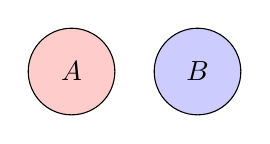
\begin{tikzpicture}[scale=0.5]
\filldraw[fill=red!20, draw=black] (-1.6,0) circle (1.1cm) node {$A$};
\filldraw[fill=blue!20, draw=black] (1.6,0) circle (1.1cm) node {$B$};
\end{tikzpicture}

\vspace{0.3cm}
\textbf{Venn Diagram} (Standard overlap template)\\
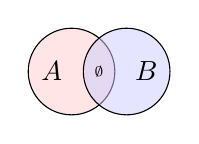
\begin{tikzpicture}[scale=0.5]
\filldraw[fill=red!20, draw=black, fill opacity=0.5] (-0.7,0) circle (1.1cm);
\filldraw[fill=blue!20, draw=black, fill opacity=0.5] (0.7,0) circle (1.1cm);
\node at (-1.2,0) {$A$};
\node at (1.2,0) {$B$};
\node at (0,0) {\tiny $\emptyset$};
\end{tikzpicture}
\end{column}
\end{columns}
\end{frame}

\begin{frame}{}
\addfig{0.5}{set_venn}{Can you guess what each set is?}{}
\end{frame}

\begin{frame}{Empty set and size}
\begin{defn}{}{}
\begin{itemize}
\item $\emptyset = \{\}$ is called the \textbf{empty set}, meaning it has no element. 
\item $|A|$ (the \textbf{size} of $A$) is the cardinality (or the number of elements) of $A$. This can either be \begin{itemize}
\item zero (if $A$ is empty)
\item a positive integer ($1,2,3,\ldots$)
\item an infinity ($\infty$)
\end{itemize}
\end{itemize}
\end{defn}
\end{frame}

\begin{frame}[t]
\begin{ex}
Express the following sets in set notation, and also find its size.
\begin{itemize}
\item The set of letters in English alphabet.
\item The set of planets in the solar system.
\item The set of odd positive integers less than 10
\item The set of integers whose square ends with digit 3.
\end{itemize}
\end{ex}
\begin{sol}
\begin{itemize}
\item $A = \{a,b,c,\ldots,z\}$ and $|A| = 26$
\item $B = \{$Earth, Jupiter, Neptune, Mars, Uranus, Saturn, Venus, Mercury$\}$ and $|B| = 8$ (Bye, Pluto)
\item $C = \{1,3,5,7,9\}$ and $|C| = 5$
\item $D = \{\}$ and $|D| = 0$
\end{itemize}
\end{sol}
\end{frame}

\begin{frame}
\frametitle{Set Comparison}
\begin{defn}{}{}
\begin{itemize}
\item $A \subseteq B$ ($A$ is a subset of $B$) if every element of $A$ is also an element of $B$. 
\item $A = B$ ($A$ is equal to $B$) if all elements in $A$ and $B$ match. 
\item $A$ and $B$ are \textbf{disjoint} if they share no elements ($A \cap B = \emptyset$).
\end{itemize}
\end{defn}
\begin{remark}{}{}
Some textbooks use the notation $A \subset B$ to imply that $A \subseteq B$ but $A \neq B$. 
\end{remark}
\end{frame}

\begin{frame}{Venn Diagrams: Subset vs. Disjoint}
\begin{columns}
\begin{column}{0.5\textwidth}
\centering
\textbf{Subset ($A \subseteq B$)}\\
\vspace{0.2cm}
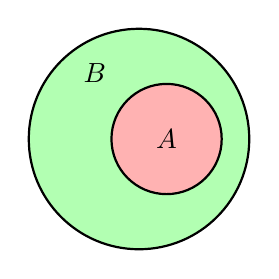
\begin{tikzpicture}[thick, scale=0.7]
\filldraw[fill = green!30!white] (0,0) circle (20mm);
\filldraw[fill = red!30!white] (0.5,0) circle (10mm);
\node at (-0.8,1.2) {$B$}; 
\node at (0.5,0) {$A$};
\end{tikzpicture}
\end{column}
\begin{column}{0.5\textwidth}
\centering
\textbf{Disjoint Sets ($A \cap B = \emptyset$)}\\
\vspace{0.2cm}
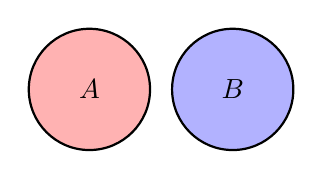
\begin{tikzpicture}[thick, scale=0.7]
\filldraw[fill = red!30!white] (-1.3,0) circle (11mm) node {$A$};
\filldraw[fill = blue!30!white] (1.3,0) circle (11mm) node {$B$};
\end{tikzpicture}
\end{column}
\end{columns}
\end{frame}

\begin{frame}[t]
\begin{ex}
For each pair of sets, determine whether they have subset ($\subseteq$), equality ($=$), disjoint ($\cap = \emptyset$), or neither relationship.
\begin{itemize}
\item $F$ = a set of fruits, $P$ = a set of plants
\item $A = \{1,2,3\}, B = \{4,3,2,1\}$
\item $W$ = Warrior skills, $M$ = Mage skills
\end{itemize}
\end{ex}
\begin{sol}
\begin{itemize}
\item $F \subseteq P$ because all fruits are plants.
\item $A \subseteq B$ because each element in $A$ - namely 1,2, and 3 - are in $B$.
\item $W \cap M = \emptyset$ if warrior and mage have completely disjoint skill sets.
\end{itemize}
\end{sol}
\end{frame}

%%%%%%%%%%%%%
\section{Set Operation}
\frame{\sectionpage}
%%%%%%%%%%%%%

\begin{frame}
\frametitle{Set Operations: Intersection}
\begin{defn}{}{}
$A \cap B$ ($A$ intersects $B$) is the set of elements that are in both $A$ and $B$. 
\end{defn}
\begin{figure}[h!]
\centering
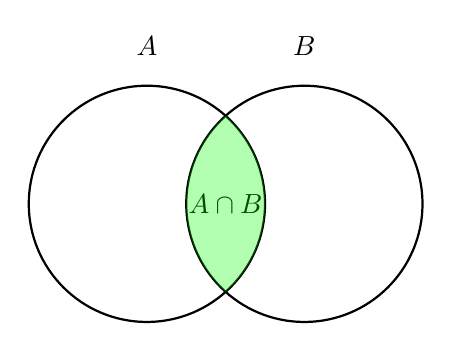
\begin{tikzpicture}[thick]
\draw (0,0) circle (15mm);
\draw (2,0) circle (15mm);
\node at (0,2) {$A$}; 
\node at (2,2) {$B$};
\node at (1,0) {$A \cap B$};
  \clip (0, 0)  circle (15mm);
  \fill[green, fill opacity = 0.3] (2,0)  circle (15mm);
\end{tikzpicture}
\caption{Venn diagram for $A$ intersects $B$}
\end{figure}
\end{frame}

\begin{frame}
\addfig{0.8}{venn_diagram_cecilia}{\href{https://www.youtube.com/watch?v=p0quM2txQwg}{Vein's diagram done... right?}}
\end{frame}

\begin{frame}
\frametitle{Set Operations: Union}
\begin{defn}{}{}
$A \cup B$ ($A$ unions $B$) is the set of elements that are in either $A$ or $B$ (or both). 
\end{defn}
\begin{figure}[h!]
\centering
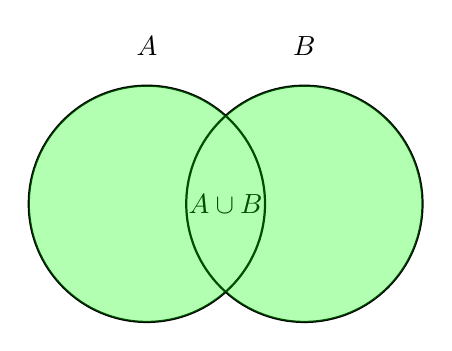
\begin{tikzpicture}[thick]
\draw (0,0) circle (15mm);
\draw (2,0) circle (15mm);
\node at (0,2) {$A$}; 
\node at (2,2) {$B$};
\node at (1,0) {$A \cup B$};
\fill[green, fill opacity = 0.3] (2,0)  circle (15mm) (0,0)  circle (15mm);
\end{tikzpicture}
\caption{Venn diagram for $A$ unions $B$}
\end{figure}
\end{frame}


\begin{frame}[t]
\begin{ex}
Let $A = \{1,2,4\}$ and $B = \{2,3,5\}$.  Find
\[A \cap B, \quad A \cup B, \quad A \setminus B, \quad B \setminus A\]
\end{ex}
\begin{sol}
\begin{itemize}
\item $A \cap B = \{2\}$ because $2$ is the only element in both $A$ and $B$. 
\item $A \cup B = \{1,2,3,4,5\}$. Note that we do not include the extra 2 as we only care about the existence, not quantity. 
\item $A \setminus B = \{1,4\}$.
\item $B \setminus A = \{3,5\}$.
\end{itemize}

\begin{figure}[h!]
\centering
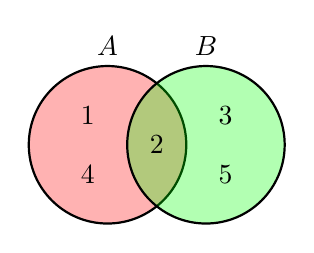
\begin{tikzpicture}[thick, scale=0.5]
\node at (0,2.5) {$A$};
\node at (2.5,2.5) {$B$};
  \filldraw[fill=red, fill opacity = 0.3]  (0,0)    circle (20mm);
  \filldraw[fill=green, fill opacity = 0.3] (2.5,0)  circle (20mm);
  \node at (1.25,0) {2};
  \node at (-0.5, 0.75) {1};
  \node at (-0.5, -0.75) {4};
  \node at (3, 0.75) {3};
  \node at (3, -0.75) {5};
\end{tikzpicture}
\caption{Venn diagram for example \theexample}
\end{figure}
\end{sol}
\end{frame}


\begin{frame}[t]
\begin{ex}
Consider all single-digits $0,1,2,3,4,5,6,7,8,9$. Let $A$ be the set of single-digits  with at least one hole, and $B$ be single-digits that have reflection symmetry (look the same in the mirror).  Find
\[A \cap B, \quad A \cup B, \quad A \setminus B, \quad B \setminus A\]
\end{ex}
\begin{sol}
First we need to write out the elements of $A$ and $B$
\[ A = \{0,4,6,8,9\}, \quad B = \{0,3,8\} \]
\begin{itemize}
\item $A \cap B = \{0,8\}$ 
\item $A \cup B = \{0,3,4,6,8,9\}$ 
\item $A \setminus B = \{4,6,9\}$.
\item $B \setminus A = \{3\}$.
\end{itemize}
\end{sol}
\end{frame}

\begin{frame}
\frametitle{Universe and Complement}
\begin{defn}{}{}
\begin{itemize}
\item A \textbf{universe} is the set $U$ that we consider to be ``everything''. 
\item $A^\mathsf{c}$ or $A'$ (a complement of $A$) is everything else that is not in $A$ but is in $U$. In other words, $A^\mathsf{c} = U \setminus A$.
\end{itemize}
\end{defn}

\begin{figure}[h!]
\centering
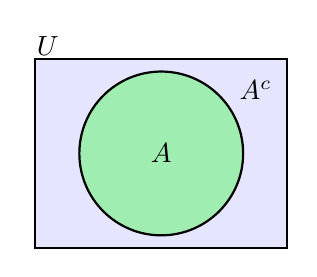
\begin{tikzpicture}[thick, scale=0.8]
\filldraw[fill = blue, fill opacity = 0.1] (0,0) rectangle (4,3);
\filldraw[fill = green, fill opacity = 0.3] (2,1.5) circle (13mm);
\node at (2,1.5) {$A$}; 
\node at (3.5,2.5) {$A^{c}$};
\node at (0.2, 3.2) {$U$};
\end{tikzpicture}
\caption{Venn diagram for set complement $A^{c}$}
\end{figure}
\end{frame}


\begin{frame}[t]
\begin{ex}
Let $A = \{1,2,3\}$. 
\begin{tasks}(1)
\task If we define $U = \{1,2,3,4,5\}$ , then find $A^\mathsf{c}$. 
\task If we define $U = \{1,2,3,8,9,10\}$ , then find $A^\mathsf{c}$.
\end{tasks}
\end{ex}
\begin{sol}
\begin{tasks}(1)
\task If we define $U = \{1,2,3,4,5\}$ , then $A^\mathsf{c} = \{4,5\}$. 
\task  If we define $U = \{1,2,3,8,9,10\}$ , then $A^\mathsf{c} = \{8,9,10\}$.
\end{tasks}
\end{sol}
\end{frame}

\begin{frame}{Game Design Application: MDA Framework}
\begin{figure}[h!]
\centering
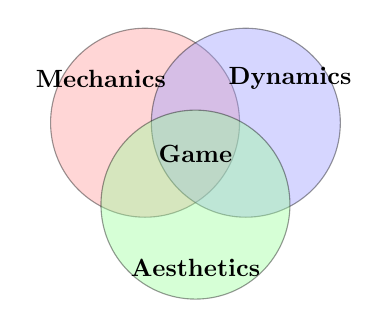
\begin{tikzpicture}[scale=0.8, every node/.style={scale=0.9}]
\filldraw[opacity=0.4, fill=red!40] (-0.8,0.5) circle (1.5cm);
\filldraw[opacity=0.4, fill=blue!40] (0.8,0.5) circle (1.5cm);
\filldraw[opacity=0.4, fill=green!40] (0,-0.8) circle (1.5cm);
\node at (-1.5,1.2) {\textbf{Mechanics}};
\node at (1.5,1.2) {\textbf{Dynamics}};
\node at (0,-1.8) {\textbf{Aesthetics}};
\node at (0,0) {\textbf{Game}};
\end{tikzpicture}
\caption{The MDA Framework: Mechanics $\cap$ Dynamics $\cap$ Aesthetics form the core player experience.}
\end{figure}
\end{frame}

%%%%%%%%%%%%%
\section{3-Set Venn Diagrams}
\frame{\sectionpage}
%%%%%%%%%%%%%

\begin{frame}{3-Set Venn Diagrams: The 8 Regions}
\begin{columns}
\begin{column}{0.5\textwidth}
A 3-set Venn diagram divides the Universe $U$ into \textbf{8 mutually exclusive regions}:
\begin{enumerate}\small
\item Center: $A \cap B \cap C$ (all 3)
\item 2-set overlaps only:
  \begin{itemize}\footnotesize
  \item $(A \cap B) \setminus C$
  \item $(B \cap C) \setminus A$
  \item $(A \cap C) \setminus B$
  \end{itemize}
\item Single set only:
  \begin{itemize}\footnotesize
  \item Only $A$, Only $B$, Only $C$
  \end{itemize}
\item Outside all sets: $(A \cup B \cup C)^\mathsf{c}$
\end{enumerate}
\end{column}
\begin{column}{0.5\textwidth}
\centering
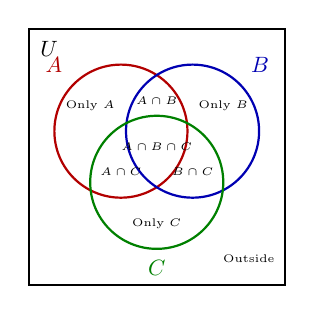
\begin{tikzpicture}[scale=0.65, every node/.style={scale=0.8}]
\draw[thick] (-2.5,-2.5) rectangle (2.5,2.5);
\node at (-2.1,2.1) {$U$};
\draw[thick, red!70!black] (-0.7,0.5) circle (1.3cm) node[above left=0.8cm] {$A$};
\draw[thick, blue!70!black] (0.7,0.5) circle (1.3cm) node[above right=0.8cm] {$B$};
\draw[thick, green!50!black] (0,-0.5) circle (1.3cm) node[below=1.1cm] {$C$};
\node at (0,0.2) {\tiny $A\cap B\cap C$};
\node at (0,1.1) {\tiny $A\cap B$};
\node at (-0.7,-0.3) {\tiny $A\cap C$};
\node at (0.7,-0.3) {\tiny $B\cap C$};
\node at (-1.3,1.0) {\tiny Only $A$};
\node at (1.3,1.0) {\tiny Only $B$};
\node at (0,-1.3) {\tiny Only $C$};
\node at (1.8,-2.0) {\tiny Outside};
\end{tikzpicture}
\end{column}
\end{columns}
\end{frame}

\begin{frame}{Constructing a 3-Set Diagram from Given Sets}
\begin{block}{Construction Strategy (Inside-Out Method)}
To correctly place elements into a 3-set Venn diagram, fill the regions from the \textbf{inside out}:
\begin{enumerate}
\item \textbf{Step 1 (Center):} Find $A \cap B \cap C$ (elements in all three sets).
\item \textbf{Step 2 (2-way overlaps):} Find remaining elements in $(A \cap B)$, $(B \cap C)$, and $(A \cap C)$.
\item \textbf{Step 3 (1-set regions):} Place remaining elements belonging exclusively to $A$, $B$, or $C$.
\item \textbf{Step 4 (Outside):} Place elements of $U$ that are not in $A \cup B \cup C$.
\end{enumerate}
\end{block}
\end{frame}

\begin{frame}[t]{Example: Constructing a 3-Set Venn Diagram}
\begin{ex}
Given $U = \{1, 2, 3, 4, 5, 6, 7, 8, 9, 10\}$ and sets:
\[ A = \{1, 2, 4, 5, 7\}, \quad B = \{2, 3, 5, 6, 8\}, \quad C = \{4, 5, 6, 7, 9\} \]
Construct the 3-set Venn diagram.
\end{ex}
\begin{sol}
\begin{columns}
\begin{column}{0.55\textwidth}
\begin{itemize}\small
\item $A \cap B \cap C = \{5\}$
\item $A \cap B \text{ (only)} = \{2\}$, $B \cap C \text{ (only)} = \{6\}$, \\ $A \cap C \text{ (only)} = \{4, 7\}$
\item Only $A = \{1\}$, Only $B = \{3, 8\}$, Only $C = \{9\}$
\item Outside $(A \cup B \cup C)^\mathsf{c} = \{10\}$
\end{itemize}
\end{column}
\begin{column}{0.45\textwidth}
\centering
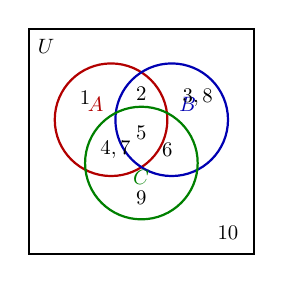
\begin{tikzpicture}[scale=0.55, every node/.style={scale=0.75}]
\draw[thick] (-2.6,-2.6) rectangle (2.6,2.6);
\node at (-2.2,2.2) {$U$};
\draw[thick, red!70!black] (-0.7,0.5) circle (1.3cm) node[above left] {$A$};
\draw[thick, blue!70!black] (0.7,0.5) circle (1.3cm) node[above right] {$B$};
\draw[thick, green!50!black] (0,-0.5) circle (1.3cm) node[below] {$C$};
\node at (0,0.2) {$5$};
\node at (0,1.1) {$2$};
\node at (-0.6,-0.2) {$4,7$};
\node at (0.6,-0.2) {$6$};
\node at (-1.3,1.0) {$1$};
\node at (1.3,1.0) {$3,8$};
\node at (0,-1.3) {$9$};
\node at (2.0,-2.1) {$10$};
\end{tikzpicture}
\end{column}
\end{columns}
\end{sol}
\end{frame}

\begin{frame}{Evaluating Set Operations visually: $A \cup (B \cap C)$}
\begin{block}{Evaluating Compound Set Operations}
Break down the operation step-by-step:
\begin{enumerate}
\item Identify the region for the inner expression: $B \cap C$ (intersection of $B$ and $C$).
\item Combine (union $\cup$) that region with the entire set $A$.
\end{enumerate}
\end{block}

\begin{figure}[h!]
\centering
\begin{subfigure}[b]{0.45\textwidth}
\centering
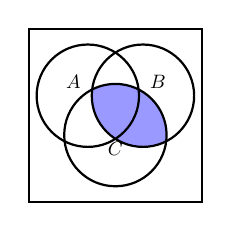
\begin{tikzpicture}[scale=0.5, every node/.style={scale=0.7}]
\draw[thick] (-2.2,-2.2) rectangle (2.2,2.2);
\begin{scope}
\clip (0.7,0.5) circle (1.3cm);
\fill[blue!40] (0,-0.5) circle (1.3cm);
\end{scope}
\draw[thick] (-0.7,0.5) circle (1.3cm) node[above left] {$A$};
\draw[thick] (0.7,0.5) circle (1.3cm) node[above right] {$B$};
\draw[thick] (0,-0.5) circle (1.3cm) node[below] {$C$};
\end{tikzpicture}
\caption{Step 1: Region $B \cap C$}
\end{subfigure}
\hfill
\begin{subfigure}[b]{0.45\textwidth}
\centering
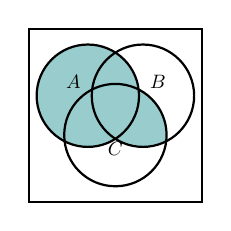
\begin{tikzpicture}[scale=0.5, every node/.style={scale=0.7}]
\draw[thick] (-2.2,-2.2) rectangle (2.2,2.2);
\fill[teal!40] (-0.7,0.5) circle (1.3cm);
\begin{scope}
\clip (0.7,0.5) circle (1.3cm);
\fill[teal!40] (0,-0.5) circle (1.3cm);
\end{scope}
\draw[thick] (-0.7,0.5) circle (1.3cm) node[above left] {$A$};
\draw[thick] (0.7,0.5) circle (1.3cm) node[above right] {$B$};
\draw[thick] (0,-0.5) circle (1.3cm) node[below] {$C$};
\end{tikzpicture}
\caption{Step 2: $A \cup (B \cap C)$}
\end{subfigure}
\end{figure}
\end{frame}

\begin{frame}{Evaluating Set Operations: More Examples}
\begin{figure}[h!]
\centering
\begin{subfigure}[b]{0.45\textwidth}
\centering
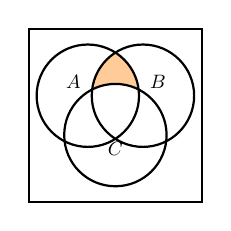
\begin{tikzpicture}[scale=0.5, every node/.style={scale=0.7}]
\draw[thick] (-2.2,-2.2) rectangle (2.2,2.2);
\begin{scope}
\clip (-0.7,0.5) circle (1.3cm);
\fill[orange!40] (0.7,0.5) circle (1.3cm);
\end{scope}
\begin{scope}
\clip (0,-0.5) circle (1.3cm);
\fill[white] (-0.7,0.5) circle (1.3cm);
\end{scope}
\draw[thick] (-0.7,0.5) circle (1.3cm) node[above left] {$A$};
\draw[thick] (0.7,0.5) circle (1.3cm) node[above right] {$B$};
\draw[thick] (0,-0.5) circle (1.3cm) node[below] {$C$};
\end{tikzpicture}
\caption{$(A \cap B) \setminus C$}
\end{subfigure}
\hfill
\begin{subfigure}[b]{0.45\textwidth}
\centering
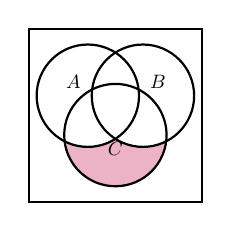
\begin{tikzpicture}[scale=0.5, every node/.style={scale=0.7}]
\draw[thick] (-2.2,-2.2) rectangle (2.2,2.2);
\fill[purple!30] (0,-0.5) circle (1.3cm);
\begin{scope}
\fill[white] (-0.7,0.5) circle (1.3cm);
\fill[white] (0.7,0.5) circle (1.3cm);
\end{scope}
\draw[thick] (-0.7,0.5) circle (1.3cm) node[above left] {$A$};
\draw[thick] (0.7,0.5) circle (1.3cm) node[above right] {$B$};
\draw[thick] (0,-0.5) circle (1.3cm) node[below] {$C$};
\end{tikzpicture}
\caption{$(A \cup B)^\mathsf{c} \cap C = C \setminus (A \cup B)$}
\end{subfigure}
\caption{Visualizing region boundaries for set operations}
\end{figure}
\end{frame}

%%%%%%%%%%%%%
\section{Activity}
\frame{\sectionpage}
%%%%%%%%%%%%%

\begin{frame}{Let's Play! Things in Rings}
\addfig{0.5}{set_things_in_rings}{Things in Rings - a board game about guessing categories using Venn diagram as a mechanics \href{https://boardgamegeek.com/boardgame/408547/things-in-rings}{: Source}}{}
\end{frame}

\begin{frame}
\frametitle{Let's Play! - Things in Rings}
\begin{figure}[h!]
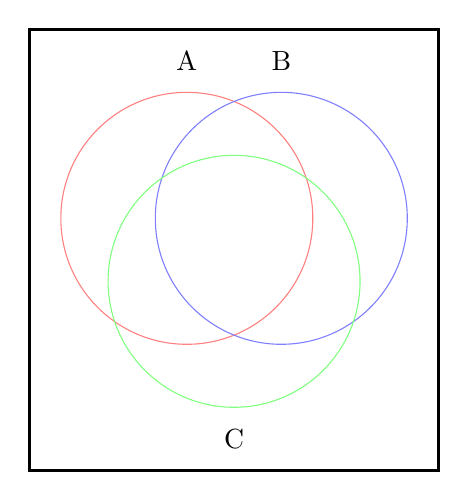
\begin{tikzpicture}[scale = 0.8]
\draw[very thick] (-2.5, -4) rectangle (4, 3);
\draw[red!50!white] (0,0) circle (20mm);
\node at (0,2.5) {A};
\draw[blue!50!white] (1.5,0) circle (20mm);
\node at (1.5, 2.5) {B};
\draw[green!50!white] (0.75,-1) circle (20mm);
\node at (0.75, -3.5) {C};
\end{tikzpicture}
\caption{A blank Venn diagram for 3 sets}
\end{figure}
\end{frame}

\begin{frame}
\frametitle{Guess My Set}
\blue{Goal}: Correctly place items three times in a row.

\blue{Set up}: 
\begin{itemize}
\item Find a game master (GM). Open \href{https://things-in-rings.vercel.app/en}{https://things-in-rings.vercel.app/en} to generate a question.
\item Split players into 3 teams.
\end{itemize}
\blue{Turn sequence}:
\begin{enumerate}
\item The active team thinks of an object, and then guess where it belongs to in the Venn diagram.
\item The GM says yes if the object is in the guessed region.
\item The active player writes down the object in the correct section on the Venn diagram.
\end{enumerate}
\blue{Game end}: The first team who correctly place items three times in a row wins! (Note that you don't need to completely determine the categories)
\end{frame}

\begin{frame}{}
\addfig{1}{set_things_in_rings_rule}{Attribute, Word and Context}{}
\end{frame}

\begin{frame}{Example}
\begin{figure}[h!]
\centering
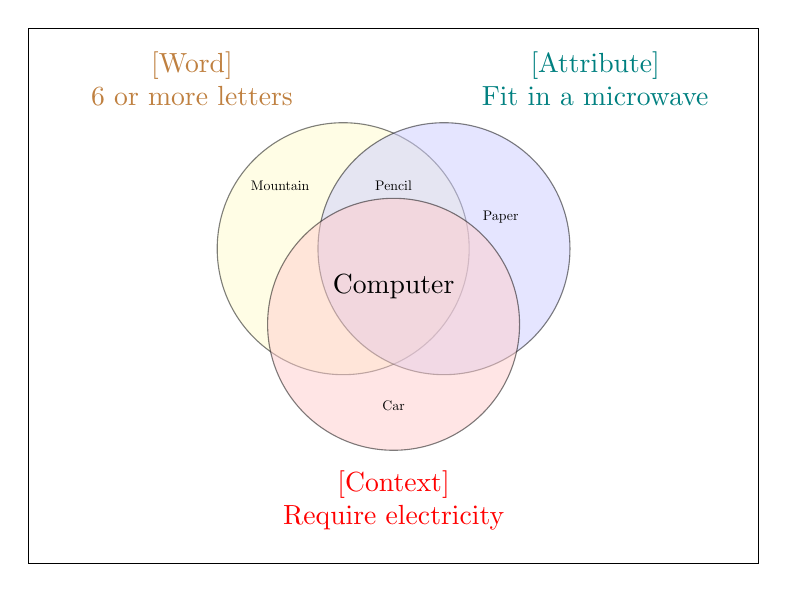
\begin{tikzpicture}[scale = 0.8]
\draw (-5, -5) rectangle (6.6,3.5);
\filldraw[opacity = 0.5, fill = yellow!20, draw = black] (0,0) circle (2cm);
\filldraw[opacity = 0.5, fill = blue!20, draw = black] (1.6,0) circle (2cm);
\filldraw[opacity = 0.5, fill = red!20, draw = black] (0.8,-1.2) circle (2cm);
\node[brown, align = center] at (-2.4,2.7) {[Word] \\ 6 or more letters};
\node[teal, align = center] at (4,2.7) {[Attribute] \\ Fit in a microwave};
\node[red, align =center] at (0.8,-4) {[Context] \\ Require electricity};
\node[scale = 0.5] at (0.8, 1) {Pencil};
\node[scale = 0.5] at (-1, 1) {Mountain};
\node[scale = 0.5] at (2.5, 0.5) {Paper};
\node[scale = 0.5] at (0.8, -2.5) {Car};
\node[scale = 1] at (0.8, -0.6) {Computer};
\end{tikzpicture}
\end{figure}
\end{frame}

\begin{frame}{}
\begin{exercisebox}{Post-play}{}
Answer the followings and submit them on Teams
\begin{itemize}
\item Take a photo of the final diagram
\item Find 2 items which goes to the center (belongs to all categories)
\item Find 2 items which goes outside the diagram (doesn't belong to any category)f
\item In your opinion, which category is the hardest? Why?
\end{itemize}
\end{exercisebox}
\end{frame}

%%%%%%%%%%%%%%%%%%%%%%%%%%%
% END
%%%%%%%%%%%%%%%%%%%%%%%%%%%
\end{document}

%%%%%%%%%%%%%
\section{Types of Sets}
\frame{\sectionpage}
%%%%%%%%%%%%%

\begin{frame}[t]
\frametitle{Types of Sets (1/3)}
Expressing the elements 
\begin{slide}
\begin{itemize}

\item Explicit: listing all elements. 

\[A = \{1,2,4\} , B = \{1,3,5,7,\ldots\}\] 
\item Implicit: stating conditions. 

\[A = \{ \text{ animals } | \text{ has four legs } \} , B = \{x \, | \, x \text{ is an even number} \}\]
\end{itemize}
\end{slide}
\end{frame}

\begin{frame}
\frametitle{Types of Sets (2/3)}
Size 
\begin{slide}
\begin{itemize}
\item Finite set: the number of elements is an integer. 

\[ A = \{ \text{atoms in the universe} \} , B = \{  \text{money you have} \}\]
\item Infinite set:  

\[ A = \{ \text{integers} \} , B = \{ \text{twin primes} \} \]
\end{itemize}
\end{slide}
\end{frame}

\begin{frame}
\frametitle{Types of Sets (3/3)}
Continuum
\begin{slide}
\begin{itemize}
\item Discrete: elements are ``apart'' from each other. 

\[ A = \{ 1,3,4,5\} \] 
\item Continuous: elements are in a range. 

\[ A = \{ \text{real numbers} \} , B = \{ x\, | \, 0 < x \leq 10 \} \]
\end{itemize}
\end{slide}
\end{frame}

\begin{frame}
\frametitle{Intervals}
There is a commonly used notation of sets called \red{interval}. This express the sets expressed by inequality signs.
\begin{defn}{}{}
\begin{eqnarray*}
[a,b] &=& \{ x \, | \, a \leq x \leq b \} \\ 
(a,b) &=& \{ x \, | \, a < x < b \} \\ 
(a,b] &=& \{ x \, | \, a < x \leq b \} \\ 
\text{[} a,b \text{)} &=& \{ x \, | \, a \leq x < b \}
\end{eqnarray*}
\end{defn}
\begin{itemize}
\item ``$($'' and ``$)$'' means non-inclusive or open. This corresponds to $<$ or $>$ signs.
\item ``$[$'' and ``$]$'' means inclusive or closed. This corresponds to $\leq$ or $\geq$ signs.
\end{itemize}
\end{frame}

\begin{frame}
\begin{figure}[h!]
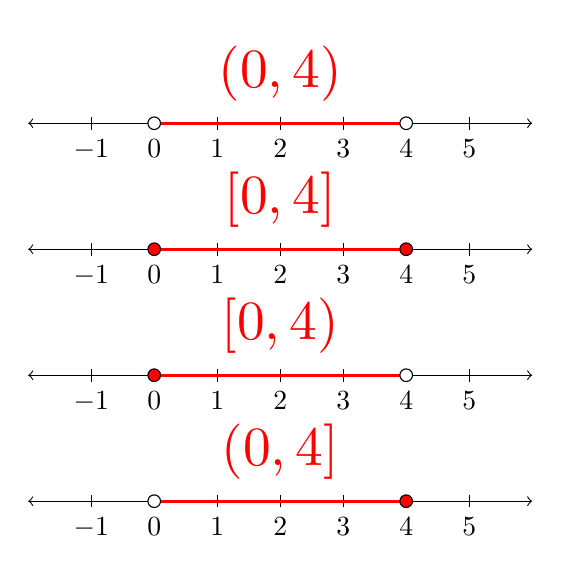
\begin{tikzpicture}[scale = 0.8]
\draw[<->] (-2,0) -- (6,0);
\foreach \x in {-1,0,...,5}
{
	\draw (\x, 0.1) -- (\x, -0.1) node [below] {$\x$};
}
\draw[red, very thick] (0,0) -- (4,0) node [pos=0.5, above, scale = 2] {$(0,4)$};
\filldraw[fill = white] (0,0) circle (1mm);
\filldraw[fill = white] (4,0) circle (1mm);

\begin{scope}[yshift = -2cm]
	\draw[<->] (-2,0) -- (6,0);
	\foreach \x in {-1,0,...,5}
	{
		\draw (\x, 0.1) -- (\x, -0.1) node [below] {$\x$};
	}
	\draw[red, very thick] (0,0) -- (4,0) node [pos=0.5, above, scale =  2] {$[0,4]$};
	\filldraw[fill = red] (0,0) circle (1mm);
	\filldraw[fill = red] (4,0) circle (1mm);
\end{scope}

\begin{scope}[yshift = -4cm]
	\draw[<->] (-2,0) -- (6,0);
	\foreach \x in {-1,0,...,5}
	{
		\draw (\x, 0.1) -- (\x, -0.1) node [below] {$\x$};
	}
	\draw[red, very thick] (0,0) -- (4,0) node [pos=0.5, above, scale = 2] {$[0,4)$};
	\filldraw[fill = red] (0,0) circle (1mm);
	\filldraw[fill = white] (4,0) circle (1mm);
\end{scope}

\begin{scope}[yshift = -6cm]
	\draw[<->] (-2,0) -- (6,0);
	\foreach \x in {-1,0,...,5}
	{
		\draw (\x, 0.1) -- (\x, -0.1) node [below] {$\x$};
	}
	\draw[red, very thick] (0,0) -- (4,0)node [pos=0.5, above, scale = 2] {$(0,4]$};
	\filldraw[fill = white] (0,0) circle (1mm);
	\filldraw[fill = red] (4,0) circle (1mm);
\end{scope}
\end{tikzpicture}
\caption{Example of interval notations. An open dot (hollow) denotes an open interval, and an opaque dot denotes a closed interval.}
\end{figure}
\end{frame}


\begin{frame}[t]
\begin{ex}
Given $A = [1,4], \quad B = (2, 5), \quad C = (3,6], \quad D = [0,7]$. Express the following set operations in terms of intervals.
\[ A \cap B, \quad B \cup C, \quad A \setminus C, \quad D \setminus C \]
\end{ex}
\begin{sol}
\begin{itemize}
\item $A \cap B = (2, 4]$
\item $B \cup C = (2,6]$
\item $A \setminus C = [1,3]$
\item $D \setminus C = [0,3] \cup (6,7]$
\end{itemize}
\end{sol}
\end{frame}

%%%%%%%%%%%%%
\section{Miscellaneous}
\frame{\sectionpage}
%%%%%%%%%%%%%

\begin{frame}
\frametitle{Other area of mathematics}
\begin{itemize}
\item Conditions 
\item Programming 
\item Combinatorics 
\item Statistics 
\item Pretty much everything
\end{itemize}
\end{frame}

\begin{frame}
\frametitle{Setception}
\addfig{0.9}{nested_sets}{Set in a set in a set in a set in a $\ldots$}
\[A = \{ \, \{ \, \{ \, \{ 1 \} \, \} \, \} \, \}\]
\end{frame}

\begin{frame}
\frametitle{Counting it Right}
A set that is nested inside another set is considered a single element. 
\begin{block}{}
Let $A = \{1, \{2\}, \{a,b,c\}\}$. Then
\begin{itemize}
\item There are 3 elements in $A$, namely the number $1$, the set $\{2\}$, and the set $\{a,b,c\}$.
\item $1 \in A$
\item $2 \not\in A$ but $\{2\} \in A$
\item $\{\{2\}\} \subseteq A$ since all elements in the set $\{\{2\}\}$ (namely $\{2\}$) are in the set $A$.
\end{itemize}
\end{block}
\end{frame}

\begin{frame}
\frametitle{Power Set}
\begin{defn}{}{}
A power set of a set $A$, denotes $P(A)$, is the set of all subsets of $A$.
\end{defn}
\addfig{0.7}{power_set}{A power set of a set with 3 elements.}
\end{frame}

\newcommand{\bt}{\bigtriangleup}
\newcommand{\bc}{\bigcirc}

\begin{frame}[t]
\frametitle{Example of Power Sets}
\begin{ex}
Find a power set of the following sets.
\[A = \{1\}, \quad B = \{\alpha, \beta\}, \quad C = \{\star, \bt, \bc\}, D = \{\}\]
\end{ex}
\begin{sol}
\begin{itemize}
\item $P(A) = \{ \emptyset, \{1\}\}$
\item $P(B) = \{ \emptyset, \{\alpha\}, \{\beta\}, \{\alpha, \beta\}\}$
\item $P(C) = \{ \emptyset, \{\star\}, \{\bt\}, \{\bc\}, \{\star, \bt\}, \{\star, \bc\}, \{\bt, \bc\}, \{\star, \bt, \bc\}\}$
\item $P(D) = \{ \emptyset\}$
\end{itemize}
\end{sol}
\end{frame}

\begin{frame}{Game Application: Crafting \& Power Sets}
\begin{block}{Item Crafting Combinations}
Let available crafting ingredients $I = \{\text{Herb}, \text{Mushroom}, \text{Crystal}\}$.
\end{block}
The power set $P(I)$ yields all $2^3 = 8$ possible ingredient combinations:
\begin{align*}
P(I) = \{ & \emptyset \text{ (No item)}, \{\text{Herb}\}, \{\text{Mushroom}\}, \{\text{Crystal}\}, \\
& \{\text{Herb}, \text{Mushroom}\}, \{\text{Herb}, \text{Crystal}\}, \{\text{Mushroom}, \text{Crystal}\}, \\
& \{\text{Herb}, \text{Mushroom}, \text{Crystal}\} \}
\end{align*}
\tcblower
\textbf{Game Design Takeaway:} Each subset in $P(I)$ maps to a unique crafted item (e.g., Potion, Elixir, Bomb, or Failed Sludge for $\emptyset$).
\end{frame}

\begin{frame}
\frametitle{Board Games!}
\addfig{0.7}{card_game_set}{\href{https://setwithfriends.com/}{Set (card game)}}
\end{frame}

\begin{frame}
\frametitle{Game Mechanic: Set Collection}
\addfig{0.6}{board_game_set_pizza_master}{An example of a set collection game: Pizza Master}
\end{frame}
